\chapter{Polynomials I: Basics and Operations}


\section{Introduction to Polynomials}
Watch Khan Academy's \textbf{Polynomials intro} video at \url{https://youtu.be/Vm7H0VTlIco}\index{polynomial}

A \emph{monomial}\index{monomial} is the product of a number and a variable raised to a non-negative (but possibly zero) integer power. Here are some examples of monomials:
\begin{multicols}{4}
  \begin{equation*}
    3 x^2
  \end{equation*}

  \begin{equation*}
    -2 x^{15}
  \end{equation*}

  \begin{equation*}
    \pi x^2
  \end{equation*}

  \begin{equation*}
    (3.33)x^{100}
  \end{equation*}

  \begin{equation*}
    7x
  \end{equation*}

  \begin{equation*}
    3
  \end{equation*}

  \begin{equation*}
    -\frac{2}{3}x^{12}
  \end{equation*}

  \begin{equation*}
    0
  \end{equation*}

  
\end{multicols}

The exponent is called the \emph{degree} of the monomial\index{monomial!degree}. For example, $3x^{17}$
has degree 17, $-7x$ has degree 1, and $3.2$ has degree 0 (because you can think of it as $(3.2)x^0$).\index{degree!polynomial}. The exponent cannot be $x$ (or any non-constant variable), as that becomes an \index{exponential function}exponential function rather than polynomial.\footnote{\index{quadratic}A quadratic is a polynomial with a maximum degree of 2}

The number in the product is called the \emph{coefficient}\index{monomial!coefficient}.  Example: $3x^{17}$ has a coefficient of 3, $-2x$ has a coefficient of -2, and $(3.4)x^{1000}$ has a coefficient of 3.4.\index{coefficient!polynomial}

A \emph{polynomial} \index{polynomial!definition of} is the sum of one or more monomials.  Here are some polynomials:
\begin{multicols}{3}
  \begin{equation*}
    4 x^2 + 9x + 3.9
  \end{equation*}

  \begin{equation*}
    -2 x^{10} + (3.4)x - 45x^{900} - 1
  \end{equation*}

  \begin{equation*}
    \pi x^2 + \pi x + \pi
  \end{equation*}

  \begin{equation*}
    3.3
  \end{equation*}

  \begin{equation*}
   7x + 2
  \end{equation*}

  \begin{equation*}
    3x^{20}
  \end{equation*}
\end{multicols}
We say that each monomial is a \index{term}\emph{term} of the polynomial.

$x^{-5} + 12$ is \emph{not} a polynomial because the first term has a negative exponent.

$x^{2} - 32x^{\frac{1}{2}} + x$ is \emph{not} a polynomial because the second term has a non-integer exponent.

$\frac{x + 2}{x^2 + x + 5}$ is \index{rational function}\emph{not} a polynomial because it is not just a sum of monomials.

\begin{Exercise}[title={Identifying Polynomials}, label=findpolynomials]
    \index{polynomial!identifying}Circle only the polynomials.
\begin{multicols}{3}
  \begin{equation*}
    -2 x^3 + \frac{1}{2}x + 3.9
  \end{equation*}

  \begin{equation*}
    2 x^{-10} + 4x - 1
  \end{equation*}
  
  \begin{equation*}
    (4.5)x^2 + \pi x
  \end{equation*}
  
  \begin{equation*}
    x^{\frac{2}{3}}
  \end{equation*}
  
  \begin{equation*}
   7
  \end{equation*}

  \begin{equation*}
    3x^{20} + 2x^{19} -5 x^{18}
  \end{equation*}
\end{multicols}
\end{Exercise}

\begin{Answer}[ref=findpolynomials]
\begin{multicols}{3}
  \begin{equation*}
    \boxed{-2 x^3 + \frac{1}{2}x + 3.9}
  \end{equation*}

  \begin{equation*}
    2 x^{-10} + 4x - 1
  \end{equation*}

  \begin{equation*}
    \boxed{(4.5)x^2 + \pi x}
  \end{equation*}

  \begin{equation*}
    x^{\frac{2}{3}}
  \end{equation*}

  \begin{equation*}
   \boxed{7}
  \end{equation*}

  \begin{equation*}
    \boxed{3x^{20} + 2x^{19} -5 x^{18}}
  \end{equation*}
\end{multicols}

\end{Answer}

We typically write a polynomial starting at the term with the highest
degree and proceed in decreasing order to the term with the lowest
degree:
\begin{equation*}
2 x^9 - 3x^7 + \frac{3}{4}x^3 + x^2 + \pi x -9.3
\end{equation*}
This is known as \emph{the standard form}.  The first term of the
standard form is called \index{leading term}\emph{the leading term}, and we often call the
coefficient of the leading term \index{leading coefficient}\emph{the leading coefficient}.  We
sometimes speak of the degree of the polynomial, which is just the
degree of the leading term.\index{standard form!polynomial}

\begin{Exercise}[title={Standard of a Polynomial}, label=polynomialstandardform]
  Write $21x^2 - x^3 + \pi - 1000x$ in standard form. What is the degree of this polynomial? What is its leading coefficient?
\end{Exercise}
\begin{Answer}[ref=polynomialstandardform]
  Standard form would be $-x^3 + 21x^2 - 1000x + \pi$. The degree is 3. The leading coefficient is $-1$
\end{Answer}

\begin{Exercise}[title={Evaluate a Polynomial}, label=evaluatepolynomial]
  Let $y = x^3 - 3x^2 + 10x - 12$. What is $y$ when $x$ is $4$?
\end{Exercise}
\begin{Answer}[ref=evaluatepolynomial]
  $4^3 - (3)(4^2) + (10)(4) - 12 = 64 - 48 + 40 - 12$. So $y = 44$ 
\end{Answer}

We would be remiss in our duties if we didn't mention one more thing
about polynomials: Mathematicians have defined a polynomial to be a sum
of a \emph{finite} number of monomials.

It is certainly possible to have a sum of an infinite number of monomials
like this:
\begin{equation*}
1 + \frac{1}{2}x + \frac{1}{4}x^2 + \frac{1}{8}x^3 + \frac{1}{16}x^4 + \ldots
\end{equation*}
This is an example of an \index{infinite series}\emph{infinite series}, which we don't consider
polynomials. Infinite series are interesting and useful, but we 
will not discuss them in detail until later in the course.


\section{Adding and Subtracting Polynomials}
Watch Khan Academy's \textbf{Adding polynomials} video at \url{https://youtu.be/ahdKdxsTj8E}

When adding two monomials of the same degree, you sum their coefficients:
\begin{equation*}
  7x^3 + 4x^3 = 11x^3
\end{equation*}\index{monomials!adding}

Using this idea, when adding two polynomials, you convert them into one long
polynomial, then simplify by \index{like terms}combining terms with the same degree. For example:
\begin{multline*}
  (10x^3 - 2x + 13) + (-5x^2 + 7x -12) \\
  = 10x^3 + (-2)x + 13 + (-5)x^2 + 7x + (-12) \\
  = 10x^3 + (-5)x^2 + (-2 + 7)x + (13 - 12) \\
  = 10x^3 - 5x^2 + 5x + 1
\end{multline*}\index{polynomials!adding}

\begin{Exercise}[title=Adding Polynomials Practice, label=addpns]
  Add the following polynomials:
  \Question{$2x^3 - 5x^2 + 3x - 9$ and $x^3 - 2x^2 - 2x - 9$}
  \vspace{20mm}
  \Question{$3x^5 - 5x^3 + 3x^2 - x - 3$ and $2x^4 - 2x^3 - 2x^2 + x - 9$}
  \vspace{20mm}
\end{Exercise}
\begin{Answer}[ref=addpns]$3x^3 - 7x^2 + x - 18$ and $3x^5 - 7x^3 + x^2 - 12$\end{Answer}

Notice that in the second question, the degree 1 term disappears completely: $(-x) + x = 0$

One more tricky thing can happen --- sometimes the coefficients don't add nicely.  For example:
\begin{equation*}
  \pi x^2 - 3 x^2 = (\pi - 3) x^2
\end{equation*}
That is as far as you can simplify it.
    
\subsection{Subtraction}
\index{polynomials!subtracting}
Now, watch Khan Academy's \textbf{Subtracting polynomials} at \url{https://youtu.be/5ZdxnFspyP8}.

When subtracting one polynomial from the other, it is a lot like
adding two polynomials. The difference: when making the two polynomials
into one long polynomial, we multiply each monomial that is being
subtracted by -1. For example:
\begin{multline*}
  (2x^2 - 3x + 9) - (5x^2 - 7x + 4) \\
  = 2x^2 + (-3)x + 9 + (-5)x^2 + 7x + (-4) \\
  = (2 - 5)x^2 + (-3 + 7)x + (9-4) \\
  = -3x^2 + 4x + 5
\end{multline*}

\begin{Exercise}[title=Subtracting Polynomials Practice, label=subtractpns]
  Subtract the following polynomials:
  \Question{$(2x^3 - 5x^2 + 3x - 9) - (x^3 - 2x^2 - 2x - 9)$}
  \vspace{20mm}
  \Question{$(3x^5 - 5x^3 + 3x^2 - x - 3) - (2x^4 - 2x^3 - 2x^2 + x - 9)$}
  \vspace{20mm}
\end{Exercise}
\begin{Answer}[ref=subtractpns]$x^3 - 3x^2 + 5x$ and $x^5 - 3x^3 + 5x^2 - 2x + 6$\end{Answer}

\subsection{Adding Polynomials in Python}\index{polynomial!adding in Python}

As a reminder, in our Python code, we are representing a \index{polynomial!list representation}polynomial
with a list of coefficients.  The first coefficient is the constant
term. The last coefficient is the leading coefficient. So, we can
imagine $-5x^3 + 3x^2 - 4x + 9$ and $2x^3 +4x^2 - 9$ would look
like this: \textit{FIXME: Diagram here}

To add the two polynomials then, we sum the coefficients for each degree.
\textit{FIXME: Diagram here}

Create a file called \filename{add\_polynomials.py}, and type in the following: 
\begin{minted}{python}
def add_polynomials(a, b):
    degree_of_result = len(a)
    result = []
    for i in range(degree_of_result):
        coefficient_a = a[i]
        coefficient_b = b[i]
        result.append(coefficient_a + coefficient_b)
    return result

polynomial1 = [9.0, -4.0, 3.0, -5.0]
polynomial2 = [-9.0, 0.0, 4.0, 2.0]
polynomial3 = add_polynomials(polynomial1, polynomial2)

print('Sum =', polynomial3)
\end{minted}

Run the program.

Unfortunately, this code only works if the polynomials are the same length. For
example, try making \pyvar{polynomial1} have a larger degree than
\pyvar{polynomial2}:
\begin{minted}{python}
# x**4 - 5x**3 + 3x**2 - 4x + 9
polynomial1 = [9.0, -4.0, 3.0, -5.0, 1.0]
  
# 2x**3 + 4x**2 - 9  
polynomial2 = [-9.0, 0.0, 4.0, 2.0]
polynomial3 = add_polynomials(polynomial1, polynomial2)
print('Sum =', polynomial3)
\end{minted}

See the problem?

\begin{Exercise}[title=Dealing with polynomials of different degrees, label=pyaddpolys]
  
\index{polynomial!different degrees}Can you fix the function \pyfunction{add\_polynomials} to handle polynomials of different degrees?

Here is a hint: In Python, there is a \pyfunction{max} function that returns the largest of the numbers it is passed.
\begin{minted}{python}
biggest = max(5,7)
\end{minted}
Here \pyvar{biggest} would be set to 7.

Here is another hint: If you have an array \pyvar{mylist}, \pyvar{i},
a non-negative integer, is only a legit index if \texttt{i <
  len(mylist)}.
\end{Exercise}
\begin{Answer}[ref=pyaddpolys]
\begin{minted}{python}
def add_polynomials(a, b):
    degree_of_result = max(len(a), len(b))
    result = []
    for i in range(degree_of_result):
        if i < len(a):
            coefficient_a = a[i]
        else:
            coefficient_a = 0.0   

        if i < len(b):
            coefficient_b = b[i]
        else:
            coefficient_b = 0.0
            
        result.append(coefficient_a + coefficient_b)
    return result
\end{minted}
\end{Answer}

\index{scalar multiplication}\section{Scalar multiplication of  polynomials}

If you multiply a polynomial with a number, the distributive property applies:
\begin{equation*}
  (3.1)(2x^2 + 3x + 1) = (6.2)x^2 + (9.3)x + 3.1
\end{equation*}
(When we are talking about things that are more complicated than a number, we use the word \index{scalar}\emph{scalar} to mean ``Just a number''. This is the product of a scalar and a polynomial.)

In \filename{add\_polynomials.py}, add a function to that multiplies a scalar and a polynomial:
\begin{minted}{python}
def scalar_polynomial_multiply(s, pn):
    result = []
    for coefficient in pn:
        result.append(s * coefficient)
    return result
\end{minted}

Somewhere near the end of the program, test this function:
\begin{minted}{python}
polynomial4 = scalar_polynomial_multiply(5.0, polynomial1)
print('Scalar product =', polynomial_to_string(polynomial4))
\end{minted}

\begin{Exercise}[title=Subtract polynomials in Python, label=pysubpoly]
Now, implement a function that does \index{polynomial!subtracting in Python}subtraction using
\pyfunction{scalar\_polynomial\_multiply} and
\pyfunction{add\_polynomials}.

It should look like this:
\begin{minted}{python}
def subtract_polynomial(a, b):
    ...Your code here...

polynomial5 = [9.0, -4.0, 3.0, -5.0]
polynomial6 = [-9.0, 0.0, 4.0, 2.0, 1.0]
polynomial7 = subtract_polynomial(polynomial5, polynomial6)
print('Difference =', polynomial_to_string(polynomial7))
\end{minted}
\end{Exercise}
\begin{Answer}[ref=pysubpoly]
\begin{minted}{python}
def subtract_polynomial(a, b):
    neg_b = scalar_polynomial_multiply(-1.0, b)
    return add_polynomials(a, neg_b)
\end{minted}
\end{Answer}


    


\section{Multiplying Polynomials}
Watch Khan Academy's \textbf{Multiplying monomials} at \url{https://www.youtube.com/watch?v=7EplN4Ch98Q}.

To review, when you multiply two monomials, you take the product of
their coefficients and the sum of their degrees:
\begin{equation*}
  (2x^6)(5x^3) = (2)(5)(x^6)(x^3) = 10x^9
\end{equation*}
If you have a product of more than two monomials, multiply \emph{all}
the coefficients and sum \emph{all} the exponents:
\begin{equation*}
  (3x^2)(2x^3)(4x) = (3)(2)(4)(x^2)(x^3)(x^1) = 24x^6
\end{equation*}\index{polynomials!multiplication}

\index{monomials!multiplication}
\begin{Exercise}[title={Multiplying monomials}, label=multmonomials]
Multiply these monomials:
  \Question $(3x^2)(5x^3)$
\vspace{20mm}
  \Question $(2x)(4x^9)$
\vspace{20mm}
  \Question $(-5.5x^2)(2x^3)$
\vspace{20mm}
  \Question $(\pi)(-2x^5)$
\vspace{20mm}
  \Question $(2x)(3x^2)(5x^7)$
\vspace{20mm}
\end{Exercise}
\begin{Answer}[ref=multmonomials]
  $(3x^2)(5x^3) = 15x^5$
  
  $(2x)(4x^9) = 8x^{10}$
  
  $(-5.5x^2)(2x^3) = -11x^5$

  $(\pi)(-2x^5) = -2\pi x^5$
  
  $(2x)(3x^2)(5x^7) = 30x^{10}$
\end{Answer}

\subsection{Multiplying a monomial and a polynomial}

Watch Khan Academy's \textbf{Multiplying monomials by polynomials} at \url{https://youtu.be/pD2-H15ucNE}.
\index{monomials!multiplying polynomials by}
When multiplying a monomial and a polynomial, you use the \index{distributive property}distributive property. After that, it is just multiplying several pairs of monomials:
\begin{multline*}
  (3x^2)(4x^3 - 2x^2 + 3x - 7) \\
  = (3x^2)(4x^3) + (3x^2)(-2x^2) + (3x^2)(3x) + (3x^2)(-7) \\
  = 12x^5 - 6x^4 + 9x^3 -21x^2
\end{multline*}

\begin{Exercise}[title={Multiplying a monomial and a polynomial}, label=multmonopoly]
Multiply these monomials:
\Question $(3x^2)(5x^3 - 2x + 3)$
\vspace{20mm}
\Question $(2x)(4x^9 - 1)$
\vspace{20mm}
\Question $(-5.5x^2)(2x^3 + 4x^2 + 6)$
\vspace{20mm}
\Question $(\pi)(-2x^5 + 3x^4 + x)$
\vspace{20mm}
\Question $(2x)(3x^2)(5x^7 + 2x)$
\end{Exercise}
\begin{Answer}[ref=multmonopoly]
  $(3x^2)(5x^3 - 2x + 3) = 15x^6 - 6x^3 + 6x^2$

  $(2x)(4x^9 - 1) = 8x^{10} - 2x$

  $(-5.5x^2)(2x^3 + 4x^2 + 6) = 11x^5 - 22x^4 + 33x^2$

  $(\pi)(-2x^5 + 3x^4 + x) = -2\pi x^5 + 3\pi x^4 + \pi x$

  $(2x)(3x^2)(5x^7 + 2x) = 30x^{10} + 12x^4$
\end{Answer}

\subsection{Multiplying polynomials}

Watch Khan Academy's \textbf{Multiplying binomials by polynomials} video at \url{https://youtu.be/D6mivA_8L8U}

When you are multiplying two polynomials, you will use the
distributive property several times to make it one long
polynomial. You will then \index{like terms}combine the terms with the same degree. For
example,
\begin{multline*}
  (2x^2 - 3)(5x^2 + 2x - 7) \\
  =   (2x^2)(5x^2 + 2x - 7) + (-3)(5x^2 + 2x - 7) \\
  =   (2x^2)(5x^2) + (2x^2)(2x) + (2x^2)(-7) + (-3)(5x^2) + (-3)(2x) + (-3)(-7) \\
  =   10^4 + 4x^3 + -14x^2 + -15x^2 + -6x + 21
  =   10^4 + 4x^3 + -29x^2 + -6x + 21
\end{multline*}

One common form that you will see is \index{binomial!multiplying}multiplying two binomials together:
\begin{multline*}
(2x + 7)(5x + 3) = (2x)(5x + 3) + (7)(5x+3) = (2x)(5x) + (7)(5x) + (2x)(3) + (7)(3)
\end{multline*}
Notice the product has become the sum of four parts: the firsts, the
inners, the outers, and the lasts. People sometimes use the mnemonic
\index{FOIL}FOIL to remember this pattern, but there is a general rule that works
for all product of polynomials, not just binomials: Every
term in the first will be multiplied by every term in the second, and
then just add them together.

So, for example, if you have a polynomial $s$ with three terms and you
multiply it by a polynomial $t$ with five terms, you will get a sum of
15 terms --- each term is a product of two monomials, one from $s$ and
one from $t$.  (Of course, several of those terms might have the same
degree, so they will be combined together when you simplify. Thus you
typically end up with a polynomial with less than 15 terms.)

Using this rule, \index{polynomial!multiplying}here is how you would multiply $2x^2 - 3x + 1$ and
$5x^2 + 2x - 7$:
\begin{multline*}
  (2x^2 - 3x + 1)(5x^2 + 2x - 7)  = \begin{matrix}
  (2x^2)(5x^2)& + &(2x^2)(2x)& + &(2x^2)(-7)& + \\
  (-3x)(5x^2)& + &(-3x)(2x)& + &(-3x)(-7)& + \\
    (1)(5x^2)& + &(1)(2x)& + &(1)(-7)& 
  \end{matrix} \\
  = 10x^4 + 4x^3 + (-14)x^2 + (-15)x^3 + (-6)x^2 + 21x +5x^2 + 2x + (-7) \\
  = 10x^4 + (4 - 15)x^3 + (-14 - 6 + 5)x^2  + (21 + 2)x + (-7) \\
  = 10x^4 - 11x^3 - 15x^2 + 23x - 7
\end{multline*}
Note that the product (before combining terms with the same degree) has
$3 \times 3 = 9$ terms --- every possible combination of a term from the
first polynomial and a term from the second polynomial.

\index{negative coefficients}One common source of error is losing track of the negative
signs. You will need to be really careful. We have found that it
helps to use + between all terms, and use negative coefficients to
express subtraction. For example, if the problem says $4x^2 - 5x - 3$,
you should work with that as $4x^2 + (-5)x + (-3)$.

\begin{Exercise}[title={Multiplying polynomials}, label=multpolys]
  Multiply the following pairs of polynomials:
  \Question{$2x + 1$ and $3x - 2$}
  \vspace{15mm}
  \Question{$-3x^2 + 5$ and $4x -2$}
  \vspace{15mm}
  \Question{$-2x - 1$ and $-3x - \pi$}
  \vspace{15mm}
  \Question{$-2x^5 + 5x$ and $3x^5 + 2x$}
  \vspace{15mm}

\end{Exercise}
\begin{Answer}[ref=multpolys]
  $(2x + 1)(3x - 2) = 6x^2 - x - 2$

  $(-3x^2 + 5)(4x - 2) = -12x^3 + 6x^2 + 20x - 10$

  $(-2x - 1)(-3x - \pi) = 6x^2 + (4 + 2\pi)x + \pi$ 

  $(-2x^5 + 5x)(3x^5 + 2x) = -6x^{10} + 12x^6 + 10x^2$
\end{Answer}

\begin{Exercise}[title={Observations}, label=obsmultpoly]
  Let's say you have two polynomials, $p_1$ and $p_2$.  $p_1$ has degree
  23.  $p_2$ has degree 12.  What is the \index{degree!of a product}degree of their product?
\end{Exercise}
\begin{Answer}[ref=obsmultpoly]
  The degree of the product is determined by the term that is the
  product of the highest degree term in $p_1$ and the highest degree
  term in $p_2$. Thus, the product of a degree 23 polynomial and a
  degree 12 polynomial has degree 35.
\end{Answer}
  


\section{Multiplying Polynomials in Python}
At this point, you have created a nice toolbox of functions for
dealing with lists of coefficients as polynomials. Create a file called \filename{poly.py} and copy the following functions into it:
\begin{itemize}
\item \pyfunction{evaluate\_polynomial}
\item \pyfunction{polynomial\_to\_string}
\item \pyfunction{add\_polynomials}
\item \pyfunction{scalar\_polynomial\_multiply}
\item \pyfunction{subtract\_polynomial}
\end{itemize}

Now, create another file in the same directory called \filename{test.py}. Type this into that file:
\begin{minted}{python}
import poly

polynomial_a = [9.0, -4.0, 3.0, -5.0]
print('Polynomial A =', poly.polynomial_to_string(polynomial_a))

polynomial_b = [-9.0, 0.0, 4.0, 2.0, 1.0]
print('Polynomial B =', poly.polynomial_to_string(polynomial_b))

# Evaluation
value_of_b = poly.evaluate_polynomial(polynomial_b, 3)
print('Polynomial B at 3 =', value_of_b)

# Adding
a_plus_b = poly.add_polynomials(polynomial_a, polynomial_b)
print('A + B =', poly.polynomial_to_string(a_plus_b))

# Scalar multiplication
b_scalar = poly.scalar_polynomial_multiply(-3.2, polynomial_b)
print('-3.2 * Polynomial B =', poly.polynomial_to_string(b_scalar))

# Subtraction
a_minus_b = poly.subtract_polynomial(polynomial_a, polynomial_b)
print('A - B =', poly.polynomial_to_string(a_minus_b))
\end{minted}

When you run it, you should get the following:
\begin{minted}{python}
Polynomial A = -5.0x^3 + 3.0x^2 + -4.0x + 9.0
Polynomial B = 1.0x^4 + 2.0x^3 + 4.0x^2 + -9.0
Polynomial B at 3 = 162.0
A + B = 1.0x^4 + -3.0x^3 + 7.0x^2 + -4.0x
-3.2 * Polynomial B = -3.2x^4 + -6.4x^3 + -12.8x^2 + 28.8
A - B = -1.0x^4 + -7.0x^3 + -1.0x^2 + -4.0x + 18.0
\end{minted}

You are now ready to implement the \index{multiply\_polynomials}multiplication of polynomials. The function will look like this:
\begin{minted}{python}
def multiply_polynomials(a, b):
  ...Your code here...
\end{minted}
It will return a list of coefficients.

In an exercise in the last chapter, you were asked `` Let's say I have
two polynomials, $p_1$ and $p_2$.  $p_1$ has degree 23.  $p_2$ has
degree 12.  What is the degree of their product?'' The answer was $23 +
12 = 35$.

In our implementation, a polynomial of degree 23 is held in a list of length 24.

In Python, we will be trying to multiply a polynomial $a$ and a
polynomial $b$ represented as lists. What is the degree of that product?
\begin{minted}{python}
result_degree = (len(a) - 1) + (len(b) - 1)
\end{minted}

Now, we need to create an array of zeros that is one longer than that. Here is a cute Python trick: If you have a list, you can \index{list!replicating}replicate it using the * operator. 
\begin{minted}{python}
a = [5,7]
b = a * 4
print(b)
# [5, 7, 5, 7, 5, 7, 5, 7]
\end{minted}

Here iss how you will get a list of zeros:
\begin{minted}{python}
result = [0.0] * (result_degree + 1)
\end{minted}

We will step through $a$, getting the index and value of each entry. You can do this in one line using \index{enumerate}\pyfunction{enumerate}:
\begin{minted}{python}
for a_degree, a_coefficient in enumerate(a):
\end{minted}
For each of those, we will step through the entire $b$ polynomial. As
you multiply together each term, you will add it to the appropriate
coefficient of the result.

Here is the whole function:
\begin{minted}{python}
def multiply_polynomials(a, b): # What is the degree of the resulting
polynomial?  result_degree = (len(a) - 1) + (len(b) - 1)

    # Make a list of zeros to hold the coefficients result = [0.0] *
    (result_degree + 1)

    # Iterate over the indices and values of a for a_degree,
    a_coefficient in enumerate(a):

        # Iterate over the indices and values of b for b_degree,
        b_coefficient in enumerate(b):

            # Calculate the resulting monomial coefficient =
            a_coefficient * b_coefficient degree = a_degree + b_degree
            
            # Add it to the right bucket
            result[degree] = result[degree] + coefficient
            
    return result
\end{minted}

Take a long look at that function.  When you understand it, type it into \filename{poly.py}.

In \filename{test.py}, try out the new function:
\begin{minted}{python}
# Multiplication
a_times_b = poly.multiply_polynomials(polynomial_a, polynomial_b)
print('A x B =', poly.polynomial_to_string(a_times_b))
\end{minted}

This is an example of a \index{nested loop}\emph{nested loop}. The outer loop steps
through the polynomial $a$. For each step it takes, the inner loop
steps through the entire polynomial $b$.

\index{aliasing}\section{Something surprising about lists}

You can imagine that you might want to create two very similar polynomials. Let's say polynomial $c$ is $x^2 + 2x + 1$ and polynomial $d$ is $x^2 -2x + 1$.  You might think you are very clever to just alter that degree 1 coefficient like this:
\begin{minted}{python}
c = [1.0, 2.0, 1.0]
d = c
d[1] = -2.0
\end{minted}

If you printed out $c$, you would get $[1.0, -2.0, 1.0]$.  Why? You
assigned two variables ($c$ and $d$) to the \emph{the same list}.  So,
when you use one reference ($d$) to change the list, you see the
change if you look at the list from either reference. \emph{FIXME:
  Diagram of two references to the same list here.}

To create two separate lists, you would need \index{list!copy} to explicitly make a copy:
\begin{minted}{python}
c = [1.0, 2.0, 1.0]
d = c.copy()
d[1] = -2.0
\end{minted}


\section{Common Polynomial Products}
In math and physics, you will run into certain kinds of polynomials
over and over again. In this chapter, we will cover some
patterns that you will want to be able to recognize as you move through the sequence!

\subsection{Difference of squares}\index{difference of squares}

To start off, watch \textbf{\textit{Polynomial special products: difference of squares}} from Khan Academy at \url{https://youtu.be/uNweU6I4Icw}.

If you are asked what $(3x - 7)(3x + 7)$ is, you would use the
distributive property to expand that to $(3x)(3x) + (3x)(7) + (-7)(3x) + (-7)(7)$.
Two of the terms cancel each other, so this is $(3x)^2 - (7)^2$. This would simplify to $9x^2 - 49$

You will see this pattern often. Anytime you see $(a + b)(a - b)$, you should immediately
recognize it equals $a^2 - b^2$. (Note that the order doesn't matter: $(a - b)(a + b)$ also equals $a^2 - b^2$.)

Working the other way is important too. Any time you see $a^2 - b^2$,
that you should recognize that you can change that into the product
$(a + b)(a - b)$. Making something into a product like this is known as
\index{factoring}\emph{factoring}. You probably have done prime factorization of
numbers like $42 = 2 \times 3 \times 7$. In the next couple of
chapters, you will learn to factorize polynomials.

\begin{Exercise}[title={Difference of Squares}, label=diffsquares]
  Simplify the following products:
  \Question{$(2x - 3)(2x + 3)$}
  \Question{$(7 + 5x^3)(7 - 5x^3)$}
  \Question{$(x - a)(x + a)$}
  \Question{$(3 - \pi)(3 + \pi)$}
  \Question{$(-4x^3 + 10)(-4x^3 - 10)$}
  \Question{$(x + \sqrt{7})(x - \sqrt{7})$}
  Factor the following polynomials:
    \Question{$x^2 - 9$}
    \Question{$49 - 16x^6$}
    \Question{$\pi^2 - 25x^8$}
    \Question{$x^2 - 5$}
\end{Exercise}
\begin{Answer}[ref=diffsquares]
  $(2x - 3)(2x + 3) = 4x^2 - 9$
  
  $(7 + 5x^3)(7 - 5x^3) = 49 - 25x^6$
  
  $(x - a)(x + a) = x^2 - a^2$
  
  $(3 - \pi)(3 + \pi) = 9 - \pi^2$
  
  $(-4x^3 + 10)(-4x^3 - 10) = 16x^6 - 100$
  
  $(x + \sqrt{7})(x - \sqrt{7}) = x^2 - 7$

  $x^2 - 9 = (x + 3)(x - 3)$

  $49 - 16x^6 = (7 + 4x^3)(7 + 4^3)$
  
  $\pi^2 - 25x^8 = (\pi + 5x^4)(\pi - 5x^4)$
  
  $x^2 - 5 = (x + \sqrt{5})(x - \sqrt{5})$

\end{Answer}

We are often interested in the \index{roots of a polynomial}roots of a polynomial. That is, we want
to know ``For what values of $x$ does the polynomial evaluate to
zero?'' For example, when you deal with falling bodies, the first
question you might ask would be ``How many seconds before the hammer
hits the ground?''  Once you have factored a polynomial into
binomials, you can easily find the roots.

For example, what are the roots of $x^2 - 5$? You just factored it
into $(x + \sqrt{5})(x - \sqrt{5})$ This product is zero if and only
if one of the factors is zero. The first factor is only zero when $x$
is $-\sqrt{5}$. The second factor is zero only when $x$ is
$\sqrt{5}$. Those are the only two roots of this
polynomial.

Let's check that result. $\sqrt{5}$ is a little more than 2.2.  Using
your Python code, you can graph the polynomial:

% original code has it as poly.py, but got errors using that
\begin{minted}{python}
import poly  
import matplotlib.pyplot as plt

# x**2 - 5
pn = [-5.0, 0.0, 1.0]

# These lists will hold our x and y values
x_list = []
y_list = []

# Start at x=-3
current_x =-3.0

# End at x=3.0
while current_x < 3.0:
    current_y = poly.evaluate_polynomial(pn, current_x)

    # Add x and y to respective lists
    x_list.append(current_x)
    y_list.append(current_y)

    # Move x forward
    current_x += 0.1

# Plot the curve
plt.plot(x_list, y_list)
plt.grid(True)

#Additional graph customization (make axes visible, axes legend)
plt.axhline(0, color='black', linewidth=1)   # x-axis
plt.axvline(0, color='black', linewidth=1)   # y-axis
plt.title("Graph of y = x² - 5")
plt.xlabel("x")
plt.ylabel("y")

plt.show()
\end{minted}

You should get a plot like Figure~\ref{fig:sqrt5}.
\begin{figure}[t]
	\centering
	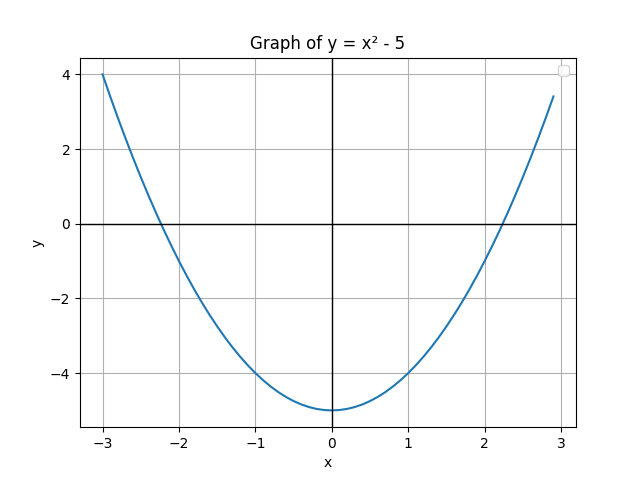
\includegraphics[width=\textwidth]{sqrt5.png}
	\caption{A graph of $x^2-5$ showing the roots on the x-axis.}
	\label{fig:sqrt5}
\end{figure}

It does, indeed, seem to cross the x-axis near -2.2 and 2.2.

\subsection{Powers of binomials}\index{binomial!powers of}

You can raise whole polynomials to exponents. Raising a polynomial to an exponent means taking the entire expression and multiplying it by itself repeatedly according to the value of the exponent. For example, 
\begin{multline*}
  (3x^3 + 5)^2 = (3x^3 + 5)(3x^3 + 5) \\ = 9x^6 + 15x^3 + 15x^3 + 25 = 9x^6 + 30x^3 + 25 
\end{multline*}

$(3x^3 + 5)^2$ is a binomial that has been raised to an exponent of 2. A polynomial with two terms is called a \index{binomial!definition of}\emph{binomial}. $5x^9 - 2x^4$,
for example, is a binomial. In this section, we are going to
develop some handy techniques for raising a binomial to some power.

Looking at the previous example, you can see that for any monomials $a$ and $b$,  
$(a + b)^2 = a^2 + 2ab + b^2.$ This is referred to as a perfect square binomial. \index{perfect squares}
So, for example, $(7x^3 + \pi)^2 = 49x^6 + 14\pi x^3 + \pi^2$

\begin{Exercise}[title={Squaring binomials}, label=squaringbinomials]
  Simplify the following
  \Question{$(x + 1)^2$}
  \Question{$(3x^5 + 5)^2$}
  \Question{$(x^3 - 1)^2$}
  \Question{$(x - \sqrt{7})^2$}
  
\end{Exercise}
\begin{Answer}[ref=squaringbinomials]
  $(x+1)^2 = x^2 + 2x + 1$

  $(3x^5 + 5)^2 = 9x^10 + 30x^5 + 25$

  $(x^3 - 1)^2 = x^6 - 2x^3 + 1$

  $(x - \sqrt{7})^2 = x^2 - 2x\sqrt{7} + 7$
\end{Answer}

What about $(x + 2)^3$? You can do it as two separate multiplications:
\begin{multline*}
  (x+2)^3 = (x+2)(x+2)(x+2) \\
  = (x + 2)(x^2 + 4x + 4) = x^3 + 4x^2 + 4x + 2x^2 + 8x + 8 \\
  = x^3 + 6x^2 + 12x + 8
\end{multline*}
In general, we can say that for any monomials $a$ and $b$, $(a + b)^3 = a^3 + 3a^2b + 3ab^2 + b^3$.

What about higher powers? $(a + b)^4$, for example? You could use the
distributive property four times, but it starts to get pretty tedious.

Here is a trick. This is known as \index{Pascal's triangle}\emph{Pascal's triangle}
\begin{equation*}
\begin{array}{c}
 1 \\
 1 \quad 1 \\
 1 \quad 2 \quad 1 \\
 1 \quad 3 \quad 3 \quad 1 \\
 1 \quad 4 \quad 6 \quad 4 \quad 1 \\
 1 \quad 5 \quad 10 \quad 10 \quad 5 \quad 1 \\
 1 \quad 6 \quad 15 \quad 20 \quad 15 \quad 6 \quad 1 \\
 1 \quad 7 \quad 21 \quad 35 \quad 35 \quad 21 \quad 7 \quad 1 \\
 \ldots
\end{array}
\end{equation*}
Each entry is the sum of the two above it.

The coefficients of each term are given by the entries in Pascal's triangle:
\begin{equation*}
(a + b)^4 = 1a^4 + 4a^3b + 6a^2 b^2 + 4 a b^3 + 1 b^4   
\end{equation*}

Notice how each term fits the form ${\displaystyle \textstyle ax^{k}y^{m}}$. The coefficient ${\displaystyle a}$ 
in each term $\textstyle ax^{k}y^{m}$ is known as the \index{binomial coefficient}binomial coefficient or \newterm{binomial theorem}. The binomial coefficient is denoted 
as ${\displaystyle \textstyle \binom{n}{k}}$ where $n$ is the exponent and $k$ is the term number (starting with 0). 
This is said ``n choose k''. \index{combinatorics} For example, in $(a + b)^4$, the coefficient of the third term 
($6a^2b^2$) is $\binom{n}{k}=\binom{4}{2} = 6$. We will heavily discuss this in a future chapter on combinatorics.

\begin{Exercise}[title={Using Pascal's Triangle}, label=pascalbinomial]
    \Question{What is $(x + \pi)^5$?}
\end{Exercise}
\begin{Answer}[ref=pascalbinomial]
  $(x + \pi)^5 = x^5 + 5\pi x^4 + 10\pi^2 x^3 + 10 \pi^3 + x^2 + 5 \pi^2 x + \pi^5$
\end{Answer}

\begin{Exercise}[title={Coding Pascal's Triangle}, label={ex:pascalrow}]

Write a Python script that finds the row of Pascal's Triangle at a given index $n$. 

\textit{Hint}: it does not need to be recursive.

\end{Exercise}

\begin{Answer}[ref={ex:pascalrow}]

\begin{minted}{python}
"""Return the nth row (0-indexed) of Pascal's Triangle."""
n = int(input("Enter row index n: "))
row = [1]
for k in range(1, n + 1):
    row.append(row[-1] * (n - k + 1) // k)
return row
\end{minted}

\end{Answer}
